\section{Assembling the linear system}
\label{sc_linearsystem}
The physical system is implemented as the mathematical differential equation in
local operators. \Dumux generates the linear system automatically. Read on, to
learn what is done internally.

\subsection{Newton's method}
The differential equations are implemented in the residual form. All terms are
on the left hand side and are summed up. The terms contain values for the primary
variables which are part of the solution vector $\textbf{u}$. The sum of the terms
is called residual $\textbf{r}(\textbf{u})$ which is a function of the solution. For
example:
\begin{align*}
\underbrace{
  \phi \frac{\partial \varrho_\alpha S_\alpha}{\partial t}
 -
 \text{div} \left(
 \varrho_\alpha \frac{k_{r\alpha}}{\mu_\alpha} \mbox{\bf K}
 \left(\grad\, p_\alpha - \varrho_{\alpha} \mbox{\bf g} \right)
 \right) - q_\alpha} _
{=: \, \textbf{r}(\textbf{u})}
= 0
\end{align*}

We don't know the solution $\textbf{u}$, so we use the iterative Newton's method to
obtain a good estimate of $\textbf{u}$. We start with an initial guess $\textbf{u}^0$ and
calculate it's residual $\textbf{r}(\textbf{u}^0)$. To minimize the error, we calculate
the derivative of the residual with respect to the solution. This is the Jacobian
matrix
\begin{align*}
  \frac{\text{d}}{\text{d}\textbf{u}}\textbf{r} \left(\textbf{u}^i\right)
  = J_{\textbf{r} \left(\textbf{u}^i\right)}
  = \left(\frac{\text{d}}{\text{d}\textbf{u}^i_m}\textbf{r} \left(\textbf{u}^i\right)_n\right)_{m,n}
\end{align*}
with $i$ denoting the Newton iteration step.
Each column is the residual derived with respect to the $m$th entry of $\textbf{u}^i$.

The Jacobian indicates the direction where the residual increases. By solving the
linear system
\begin{align*}
  J_{\textbf{r}(\textbf{u}^i)} \cdot \textbf{x}^i = \textbf{u}^i
\end{align*}
we calculate the direction of maximum growth $\textbf{x}^i$. We subtract it from
our current solution to get a new, better solution
$\textbf{u}^{i+1} = \textbf{u}^i - \textbf{x}^i$.

We repeat the calculation of of the Jacobian $J_{\textbf{r}(\textbf{u}^i)}$ and the
direction of maximum growth $\textbf{x}^i$ until our approximated solution becomes good enough.

\subsection{Structure of matrix and vectors}
To understand the meaning of an entry in the matrix or the vector of the linear system, we have
to define their structure. Both have a blocking structure. Each block contains the degrees of
freedom (also called variable or unknown) for a sub-control volume. The equation index is used
to order of the degrees of freedom. For each sub-control volume we have one block. The mapper is
used to order the blocks.

\begin{figure}[htbp]
\begin{center}
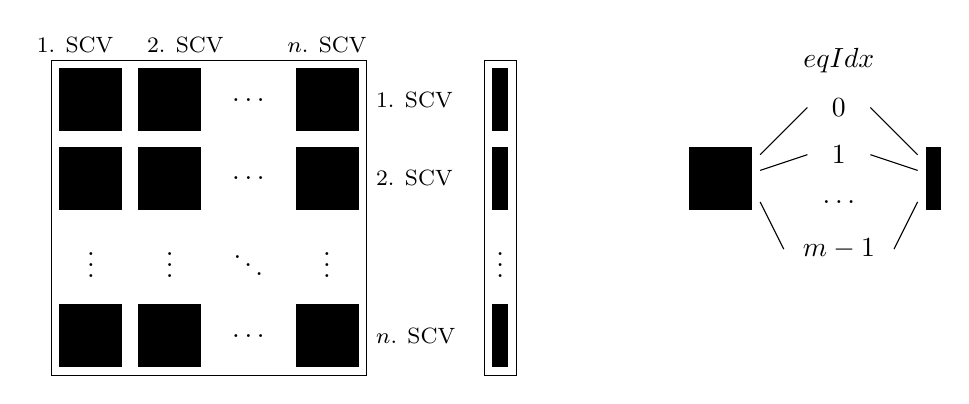
\begin{tikzpicture}
  %% blocking structure
  % matrix
  \node at (0.3,4.2){\footnotesize 1. SCV};
  \node at (1.7,4.2){\footnotesize 2. SCV};
  \node at (3.5,4.2){\footnotesize $n$. SCV};

  \draw (0,0) rectangle (4,4);
  
  \fill (0.1,3.1) rectangle (0.9,3.9);
  \fill (1.1,3.1) rectangle (1.9,3.9);
  \node at (2.5,3.5) {$\dots$};
  \fill (3.1,3.1) rectangle (3.9,3.9);
  \node at (4,3.5) [right]{\footnotesize 1. SCV};

  \fill (0.1,2.1) rectangle (0.9,2.9);
  \fill (1.1,2.1) rectangle (1.9,2.9);
  \node at (2.5,2.5) {$\dots$};
  \fill (3.1,2.1) rectangle (3.9,2.9);
  \node at (4,2.5) [right]{\footnotesize 2. SCV};

  \node at (0.5,1.5) {$\vdots$};
  \node at (1.5,1.5) {$\vdots$};
  \node at (2.5,1.5) {$\ddots$};
  \node at (3.5,1.5) {$\vdots$};

  \fill (0.1,0.1) rectangle (0.9,0.9);
  \fill (1.1,0.1) rectangle (1.9,0.9);
  \node at (2.5,0.5) {$\dots$};
  \fill (3.1,0.1) rectangle (3.9,0.9);
  \node at (4,0.5) [right]{\footnotesize $n$. SCV};

  % vector
  \draw (5.5,0) rectangle (5.9,4);
  \fill (5.6,3.1) rectangle (5.8,3.9);
  \fill (5.6,2.1) rectangle (5.8,2.9);
  \node at (5.7,1.5) {$\vdots$};
  \fill (5.6,0.1) rectangle (5.8,0.9);
  
  %% intra-block structure
  \fill (8.1,2.1) rectangle (8.9,2.9);
  \draw (9,2.8) -- (9.6,3.4);
  \draw (9,2.6) -- (9.6,2.8);
  \draw (9,2.2) -- (9.3,1.6);
  
  \node at (10,4) {${eqIdx}$};
  \node at (10,3.4) {$0$};
  \node at (10,2.8) {$1$};
  \node at (10,2.2) {$\dots$};
  \node at (10,1.6) {$m-1$};
  
  \fill (11.1,2.1) rectangle (11.3,2.9);
  \draw (11,2.8) -- (10.4,3.4);
  \draw (11,2.6) -- (10.4,2.8);
  \draw (11,2.2) -- (10.7,1.6);
\end{tikzpicture}
\end{center}
\caption{Structure of matrix and vector, left blocking structure, right within block}
\end{figure}

Accessing entries follows this structure. You can access the pressure value in the third sub-control volume in
a vector \lstinline{sol} with \lstinline{sol[2][pressureIdx]}.
